\documentclass[tikz,border=6pt]{standalone}
\usepackage{amsmath,amssymb}
\usetikzlibrary{arrows.meta,patterns}
\begin{document}
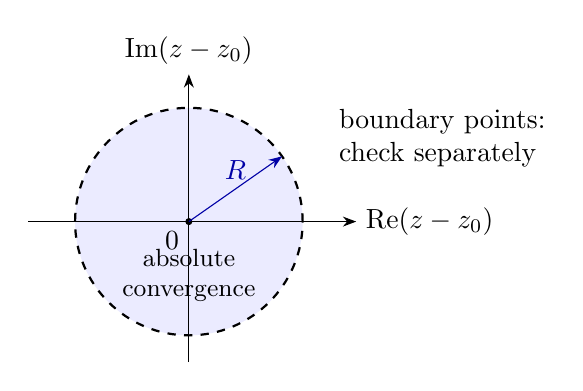
\begin{tikzpicture}[>=Stealth,scale=.85]
 \fill[blue!8] (0,0) circle (1.7);
 \draw[->] (-2.4,0)--(2.5,0) node[right]{$\operatorname{Re}(z-z_0)$};
 \draw[->] (0,-2.1)--(0,2.2) node[above]{$\operatorname{Im}(z-z_0)$};
 \draw[dashed,thick] (0,0) circle (1.7);
 \fill (0,0) circle (1.5pt) node[below left]{$0$};
 \draw[->,blue!65!black] (0,0)--(35:1.7) node[midway,above]{$R$};
 \node[align=center,font=\small] at (0,-.8) {absolute\\convergence};
 \node[right,align=left] at (2.1,1.25) {boundary points:\\check separately};
\end{tikzpicture}
\end{document}
